\documentclass[aspectratio=169]{beamer}
\usepackage{fontspec}
\usepackage[vietnamese]{babel}
\usepackage{graphicx}
\usepackage{booktabs}
\usepackage{listings}
\usepackage{caption}

% Cài đặt theme
\usetheme{Madrid}
\usecolortheme{default}
\setbeamertemplate{navigation symbols}{}
\setbeamertemplate{caption}[numbered]
\setbeamertemplate{footline}[frame number]

% Cấu hình listings cho code Python
\lstset{
    language=Python,
    basicstyle=\ttfamily\scriptsize,
    keywordstyle=\color{blue},
    stringstyle=\color{red},
    commentstyle=\color{green!60!black},
    numbers=left,
    numberstyle=\tiny\color{gray},
    stepnumber=1,
    showstringspaces=false,
    tabsize=4,
    breaklines=true,
    breakatwhitespace=true,
    frame=single,
    backgroundcolor=\color{gray!10}
}

\title[Chương 13: Tải \& Tiền Xử Lý Dữ Liệu]{Chương 13: Tải và Tiền Xử Lý Dữ Liệu với TensorFlow}
\author[Giảng viên]{Giảng viên: [Tên Giảng Viên]}
\institute[Đại Học Đông Á]{Đại Học Đông Á}
\date{\today}

\begin{document}

\begin{frame}
    \titlepage
\end{frame}

\begin{frame}{Nội dung Chương 13}
    \tableofcontents
\end{frame}

\section{1. Giới thiệu về API tf.data}

\begin{frame}{Vấn đề với dữ liệu cực lớn}
    \begin{itemize}
        \item Trong Deep Learning, chúng ta thường làm việc với tập dữ liệu (dataset) khổng lồ không thể chứa vừa trong bộ nhớ RAM.
        \item Cần một cơ chế để \textbf{tải dữ liệu dần dần (lazy loading)} từ ổ cứng, tiền xử lý trên đường đi, và đưa từng batch vào GPU một cách trơn tru.
        \item TensorFlow cung cấp \textbf{Data API (tf.data)} để giải quyết hoàn hảo bài toán này.
        \item tf.data có thể đọc từ văn bản, tệp nhị phân, hoặc cơ sở dữ liệu SQL, đồng thời hỗ trợ nén và xử lý đa luồng.
    \end{itemize}
\end{frame}

\begin{frame}[fragile]{Khởi tạo tf.data.Dataset từ Tensor}
    Cách đơn giản nhất để tạo Dataset là từ một Tensor có sẵn trên RAM:
\begin{lstlisting}[language=Python]
import tensorflow as tf

# Tao dataset tu mot tensor
X = tf.range(10) # 0, 1, 2, ..., 9
dataset = tf.data.Dataset.from_tensor_slices(X)

for item in dataset:
    print(item)
\end{lstlisting}
    \begin{itemize}
        \item Hàm \texttt{from\_tensor\_slices()} sẽ lấy tensor đầu vào và trả về một đối tượng Dataset.
        \item Mỗi phần tử của Dataset này là một phần tử của tensor ban đầu (slice dọc theo chiều thứ 0).
    \end{itemize}
\end{frame}

\begin{frame}{Các phép biến đổi chuỗi (Chaining Transformations)}
    \begin{columns}
        \begin{column}{0.5\textwidth}
            \begin{itemize}
                \item Sau khi có dataset, bạn có thể áp dụng các phép biến đổi lên nó bằng cách gọi các phương thức.
                \item Các phương thức này \textbf{không thay đổi dataset cũ} mà tạo ra một \textbf{dataset mới}.
                \item Các thao tác phổ biến: \texttt{repeat()}, \texttt{batch()}, \texttt{map()}, \texttt{filter()}.
                \item \textbf{Hình 13-1} mô tả một đường ống (pipeline) điển hình.
            \end{itemize}
        \end{column}
        \begin{column}{0.5\textwidth}
            \centering
            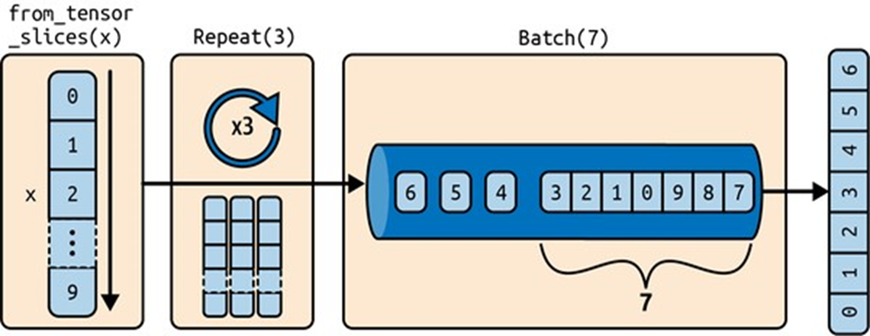
\includegraphics[width=\textwidth,height=0.7\textheight,keepaspectratio]{../machineLearningWeb/Figures/CH13/Hình_13-1}
            \vspace{0.2cm}
            \textit{Hình 13-1: Xếp chuỗi các phép biến đổi tập dữ liệu}
        \end{column}
    \end{columns}
\end{frame}

\begin{frame}[fragile]{Ví dụ: Repeat và Batch}
\begin{lstlisting}[language=Python]
# Lap lai dataset 3 lan va nhom thanh cac batch kich thuoc 7
dataset = dataset.repeat(3).batch(7)

for item in dataset:
    print(item)
\end{lstlisting}
    \begin{itemize}
        \item Output:
        \item `tf.Tensor([0 1 2 3 4 5 6], shape=(7,), dtype=int32)`
        \item `tf.Tensor([7 8 9 0 1 2 3], shape=(7,), dtype=int32)`
        \item ... (Tổng cộng 30 phần tử, chia làm 5 batch).
        \item Lệnh \texttt{drop\_remainder=True} trong \texttt{batch()} nếu muốn các batch phải bằng nhau.
    \end{itemize}
\end{frame}

\begin{frame}[fragile]{Ví dụ: Map và Filter}
    \begin{itemize}
        \item \texttt{map()}: Áp dụng một hàm lên mỗi phần tử của dataset. Thường dùng để tiền xử lý (vd: chuẩn hóa ảnh).
        \item \texttt{filter()}: Lọc bỏ các phần tử không thỏa mãn điều kiện.
    \end{itemize}
\begin{lstlisting}[language=Python]
# Nhan doi gia tri
dataset = dataset.map(lambda x: x * 2)

# Loc cac phan tu < 10
dataset = dataset.filter(lambda x: x < 10)

# Lay 3 phan tu dau tien
for item in dataset.take(3):
    print(item)
\end{lstlisting}
\end{frame}

\begin{frame}[fragile]{Trộn dữ liệu (Shuffling)}
    \begin{itemize}
        \item Thuật toán Gradient Descent hoạt động tốt nhất khi các mẫu huấn luyện hoàn toàn độc lập và được phân phối ngẫu nhiên độc lập (IID).
        \item Hàm \texttt{shuffle()} sử dụng một \textbf{buffer} để chứa các phần tử, rồi bốc ngẫu nhiên từ buffer này.
    \end{itemize}
\begin{lstlisting}[language=Python]
dataset = tf.data.Dataset.range(10).repeat(3)
dataset = dataset.shuffle(buffer_size=5, seed=42).batch(7)
\end{lstlisting}
    \begin{itemize}
        \item \textbf{Lưu ý quan trọng:} \texttt{buffer\_size} phải đủ lớn. Nếu \texttt{buffer\_size=1}, dữ liệu sẽ không bị trộn chút nào! Nếu dữ liệu lớn, cần trộn ở cấp độ file trước.
    \end{itemize}
\end{frame}

\section{2. Đọc và Tiền Xử Lý Dữ Liệu Lớn}

\begin{frame}{Quy trình làm việc với nhiều file CSV}
    \begin{columns}
        \begin{column}{0.4\textwidth}
            \begin{itemize}
                \item Khi có hàng trăm GB dữ liệu chia thành hàng ngàn file CSV:
                \begin{enumerate}
                    \item Trộn danh sách đường dẫn file (File paths).
                    \item Đọc luân phiên (Interleave) từ nhiều file cùng lúc.
                    \item Trộn dữ liệu ở cấp độ dòng (Buffer shuffle).
                    \item Phân lô (Batching).
                \end{enumerate}
                \item \textbf{Hình 13-2} mô phỏng quá trình cực kì mạnh mẽ này.
            \end{itemize}
        \end{column}
        \begin{column}{0.6\textwidth}
            \centering
            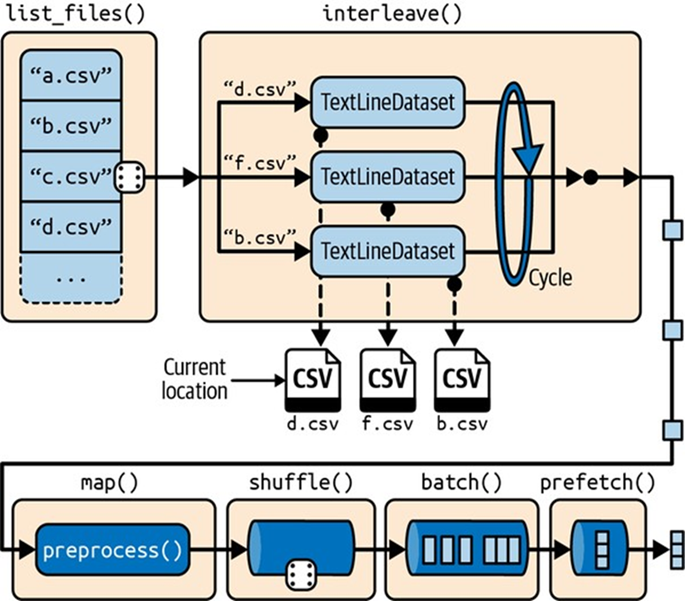
\includegraphics[width=\textwidth,height=0.65\textheight,keepaspectratio]{../machineLearningWeb/Figures/CH13/Hình_13-2}
            \vspace{0.2cm}
            \textit{Hình 13-2: Tải và tiền xử lý dữ liệu từ nhiều tệp CSV}
        \end{column}
    \end{columns}
\end{frame}

\begin{frame}[fragile]{Code: Interleave Đọc Song Song}
\begin{lstlisting}[language=Python]
filepath_dataset = tf.data.Dataset.list_files(train_filepaths, seed=42)

# interleave() se doc tu 5 file song song cung mot luc
n_readers = 5
dataset = filepath_dataset.interleave(
    lambda filepath: tf.data.TextLineDataset(filepath).skip(1), # bo qua dong Header
    cycle_length=n_readers
)

for line in dataset.take(3):
    print(line.numpy())
\end{lstlisting}
    \begin{itemize}
        \item Dữ liệu từ các file khác nhau sẽ được đan xen kẽ vào nhau.
        \item Tham số \texttt{num\_parallel\_calls=tf.data.AUTOTUNE} cho phép TF tự quyết định số luồng đọc.
    \end{itemize}
\end{frame}

\begin{frame}[fragile]{Tiền Xử Lý Dữ Liệu Từng Dòng (Preprocessing)}
    Chúng ta cần chuyển chuỗi (string) thành tensor số thực:
\begin{lstlisting}[language=Python]
n_inputs = 8 # vd: dataset California Housing co 8 dac trung

def preprocess(line):
    # Dinh nghia kieu du lieu mac dinh cho moi cot
    defs = [0.] * n_inputs + [tf.constant([], dtype=tf.float32)]
    # Phan tich chuoi CSV
    fields = tf.io.decode_csv(line, record_defaults=defs)
    x = tf.stack(fields[:-1]) # lay 8 cot dau lam X
    y = tf.stack(fields[-1:]) # cot cuoi lam Y
    # Chuan hoa X (neu da tinh san mean, std)
    return (x - X_mean) / X_std, y
\end{lstlisting}
\end{frame}

\begin{frame}{Quản lý Hiệu suất: Prefetching (Tải trước)}
    \begin{columns}
        \begin{column}{0.5\textwidth}
            \begin{itemize}
                \item Lệnh \texttt{dataset.prefetch(1)} vô cùng quan trọng.
                \item Trong khi mô hình (GPU) đang thực thi việc huấn luyện (forward/backward pass) ở Batch N.
                \item CPU sẽ tranh thủ làm việc để chuẩn bị sẵn Batch N+1 và đẩy vào bộ nhớ GPU.
                \item \textbf{Hình 13-3}: Thay vì CPU và GPU phải đợi nhau (như biểu đồ trên), chúng làm việc song song (biểu đồ dưới), tăng gấp đôi hiệu suất.
            \end{itemize}
        \end{column}
        \begin{column}{0.5\textwidth}
            \centering
            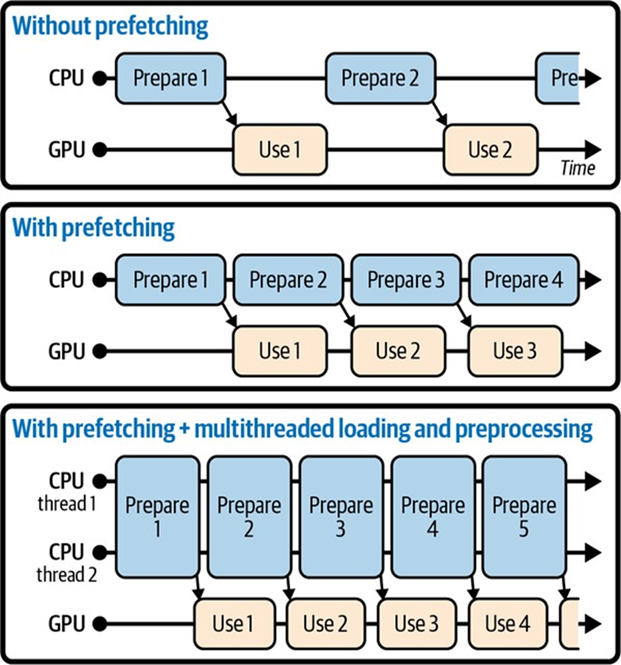
\includegraphics[width=\textwidth,height=0.7\textheight,keepaspectratio]{../machineLearningWeb/Figures/CH13/Hình_13-3}
            \vspace{0.2cm}
            \textit{Hình 13-3: Cơ chế Prefetching CPU và GPU hoạt động song song}
        \end{column}
    \end{columns}
\end{frame}

\begin{frame}{Sử dụng Dataset trong Keras}
    \begin{itemize}
        \item Keras hoàn toàn tương thích với \texttt{tf.data.Dataset}.
        \item Bạn không cần truyền $X$ và $y$ riêng lẻ, chỉ cần truyền toàn bộ \texttt{dataset} vào \texttt{fit()}.
    \end{itemize}
\end{frame}
    
\begin{frame}[fragile]{Code: Huấn luyện với tf.data}
\begin{lstlisting}[language=Python]
# Xay dung mo hinh Keras
model = keras.models.Sequential([
    keras.layers.Dense(30, activation="relu", input_shape=X_train.shape[1:]),
    keras.layers.Dense(1),
])
model.compile(loss="mse", optimizer="sgd")

# Huan luyen
model.fit(train_dataset, steps_per_epoch=len(X_train) // batch_size, 
          epochs=10, validation_data=valid_dataset)
\end{lstlisting}
\end{frame}

\begin{frame}{Ví dụ Cụ Thể Về Các Giai Đoạn Đọc Dữ Liệu}
    \begin{itemize}
        \item \textbf{Cấp độ 1:} Danh sách file. Gồm hàng ngàn file \texttt{.csv} chứa dữ liệu.
        \item \textbf{Cấp độ 2:} \texttt{interleave()}. Đọc 5 file cùng lúc. Các luồng đọc đan xen (interleave) dòng của 5 file này vào nhau.
        \item \textbf{Cấp độ 3:} \texttt{shuffle()}. Đưa các dòng vừa đọc được vào một bộ đệm (buffer). Chọn ngẫu nhiên từ bộ đệm này để đầu ra không bị lặp lại theo thứ tự file gốc.
        \item \textbf{Cấp độ 4:} \texttt{batch()}. Nhóm dữ liệu (vd: 32 dòng/batch).
        \item \textbf{Cấp độ 5:} \texttt{prefetch()}. Kéo trước batch tiếp theo.
    \end{itemize}
\end{frame}

\begin{frame}[fragile]{Giải nén TFRecord (Parsing)}
    Khi đọc TFRecord, bạn nhận được chuỗi byte thô, cần giải nén bằng \texttt{tf.io.parse\_single\_example()}:
\begin{lstlisting}[language=Python]
feature_description = {
    "name": tf.io.FixedLenFeature([], tf.string, default_value=""),
    "id": tf.io.FixedLenFeature([], tf.int64, default_value=0),
    "emails": tf.io.VarLenFeature(tf.string),
}

def parse_record(record):
    return tf.io.parse_single_example(record, feature_description)

dataset = tf.data.TFRecordDataset(["my_data.tfrecord"]).map(parse_record)
\end{lstlisting}
\end{frame}

\begin{frame}{Chuẩn Hóa Hình Ảnh (Image Standardization)}
    \begin{itemize}
        \item Khi làm việc với hình ảnh, chúng ta cần thu phóng kích thước (Resize), cắt xén (Crop) và chuẩn hóa.
        \item Keras có thư viện tiền xử lý cực tốt: \texttt{tf.keras.layers.Resizing}, \texttt{tf.keras.layers.Rescaling}.
        \item Hoặc sử dụng \texttt{tf.image} API:
        \begin{itemize}
            \item \texttt{tf.image.resize()}
            \item \texttt{tf.image.random\_crop()}
            \item \texttt{tf.image.random\_flip\_left\_right()}
        \end{itemize}
    \end{itemize}
\end{frame}

\begin{frame}[fragile]{Data Augmentation Bằng Keras Layers}
\begin{lstlisting}[language=Python]
data_augmentation = keras.models.Sequential([
    keras.layers.RandomFlip("horizontal"),
    keras.layers.RandomRotation(0.1),
    keras.layers.RandomZoom(0.2),
])
\end{lstlisting}
    \begin{itemize}
        \item Các lớp Tăng Cường Dữ Liệu (Data Augmentation) này \textbf{chỉ hoạt động trong giai đoạn huấn luyện (Training)}. 
        \item Khi mô hình dự đoán thực tế (Testing / Inference), các lớp này sẽ tự động bị tắt!
    \end{itemize}
\end{frame}

\begin{frame}{Xử Lý Văn Bản: TextVectorization}
    \begin{itemize}
        \item Tương tự \texttt{StringLookup} nhưng dành riêng cho đoạn văn bản nguyên vẹn.
        \item Nó bao gồm:
        \begin{enumerate}
            \item Làm sạch (loại bỏ dấu câu, in thường).
            \item Tách từ (Tokenization), tách bằng khoảng trắng.
            \item Lập từ điển (Build vocabulary).
            \item Mã hóa mỗi từ thành một số nguyên (index).
        \end{enumerate}
    \end{itemize}
\end{frame}

\begin{frame}[fragile]{Ví Dụ: TextVectorization}
\begin{lstlisting}[language=Python]
text_layer = keras.layers.TextVectorization()
text_layer.adapt(["Hello world!", "Machine Learning is great"])

# Bien cau sau thanh danh sach cac con so
print(text_layer(["Hello Machine"]))
\end{lstlisting}
    \begin{itemize}
        \item Đặc biệt, lớp này có thể chuyển đổi danh sách các số nguyên thành One-Hot hoặc TF-IDF.
        \item Rất hữu ích cho các mô hình NLP cơ bản.
    \end{itemize}
\end{frame}

\begin{frame}{Cơ chế Hashing (Băm Phân Loại)}
    \begin{itemize}
        \item Đôi khi biến phân loại có Quá nhiều giá trị duy nhất (vd: 50,000 danh mục) và ta không muốn lập một từ điển khổng lồ.
        \item Hoặc ta liên tục có danh mục Mới (out of vocabulary).
        \item Kỹ thuật \textbf{Hashing (Băm)}: Đưa chuỗi vào một hàm băm, giả sử ép vào 1,000 nhóm (bins).
        \item Hai danh mục khác nhau có thể bị băm vào cùng một nhóm (Collisions), nhưng nhờ Nhúng (Embedding), mạng học vẫn tìm ra cách giải quyết.
    \end{itemize}
\end{frame}

\begin{frame}[fragile]{Sử dụng HashingLayer trong Keras}
\begin{lstlisting}[language=Python]
hashing_layer = keras.layers.Hashing(num_bins=10)
# Ket qua: "Cuon sach A" -> bin 4, "Cuon sach B" -> bin 7, v.v.

encoded = hashing_layer(tf.constant(["Cuon sach A", "Cuon sach B"]))
\end{lstlisting}
    \begin{itemize}
        \item Không cần gọi \texttt{adapt()}. Không cần tạo từ điển!
        \item Cực kỳ nhanh, tốn rất ít bộ nhớ, có thể dùng on-the-fly.
    \end{itemize}
\end{frame}

\begin{frame}{TensorFlow Hub (TF Hub)}
    \begin{itemize}
        \item Thay vì tự huấn luyện một lớp Embedding cho các từ Tiếng Anh, tại sao không tải một lớp Embedding xuất sắc đã được Google huấn luyện trên hàng tỷ tài liệu?
        \item \textbf{TF Hub} là nền tảng chia sẻ các thành phần mạng nơ-ron có sẵn.
        \item Nó chứa hàng trăm mô hình nhúng văn bản (Text Embeddings) đa ngôn ngữ, mạng nhúng hình ảnh (Image Embeddings) từ ResNet.
    \end{itemize}
\end{frame}

\begin{frame}[fragile]{Cách tải Mô Hình từ TF Hub}
\begin{lstlisting}[language=Python]
import tensorflow_hub as hub

hub_layer = hub.KerasLayer("https://tfhub.dev/google/nnlm-en-dim50/2",
                           dtype=tf.string, input_shape=[], 
                           trainable=True)

model = keras.Sequential([
    hub_layer,
    keras.layers.Dense(16, activation='relu'),
    keras.layers.Dense(1, activation='sigmoid')
])
\end{lstlisting}
\end{frame}

\section{3. TFRecord Format}

\begin{frame}{Giới thiệu TFRecord}
    \begin{itemize}
        \item Text CSV rất phổ biến, nhưng tốn dung lượng và phân tích cú pháp chậm.
        \item \textbf{TFRecord} là định dạng nhị phân nhẹ, linh hoạt, do TensorFlow thiết kế.
        \item Nó chứa một chuỗi các bản ghi (records) nhị phân có kích thước linh hoạt.
        \item TFRecord có thể được nén dễ dàng (GZIP) và luồng xử lý của tf.data hoạt động cực kì nhanh với chúng.
        \item Hữu ích nhất khi lưu trữ \textbf{Hình Ảnh} hoặc \textbf{Âm thanh} kèm theo nhãn.
    \end{itemize}
\end{frame}

\begin{frame}[fragile]{Đọc và Viết TFRecord}
\begin{lstlisting}[language=Python]
# Viet
with tf.io.TFRecordWriter("my_data.tfrecord") as f:
    f.write(b"This is the first record")
    f.write(b"And this is the second record")

# Doc
filepaths = ["my_data.tfrecord"]
dataset = tf.data.TFRecordDataset(filepaths)
for item in dataset:
    print(item)
\end{lstlisting}
\end{frame}

\begin{frame}[fragile]{Protocol Buffers (Protobuf)}
    \begin{itemize}
        \item TFRecord thường chứa các Protocol Buffers (protobuf) được tuần tự hóa (serialized).
        \item Protobuf là định dạng dữ liệu mã nguồn mở của Google, tương tự JSON nhưng nhẹ hơn và xử lý siêu nhanh.
    \end{itemize}
\begin{lstlisting}[language=Python]
# Dinh nghia cau truc protobuf (file .proto)
syntax = "proto3";
message Person {
  string name = 1;
  int32 id = 2;
  repeated string email = 3;
}
\end{lstlisting}
\end{frame}

\section{4. Các Lớp Tiền Xử Lý của Keras}

\begin{frame}{Tiền Xử Lý Bằng Keras Layers}
    \begin{columns}
        \begin{column}{0.5\textwidth}
            \begin{itemize}
                \item Thay vì viết script tiền xử lý tách rời, bạn có thể \textbf{nhúng} thẳng quy trình tiền xử lý vào trong mô hình Keras!
                \item Lợi ích: Bất kì ai dùng model của bạn chỉ cần đẩy dữ liệu thô (chuỗi, ảnh gốc) vào, model tự xử lý rồi dự đoán.
                \item \textbf{Hình 13-4}: Mô hình tích hợp cả các lớp như Standardization, Text Vectorization ngay bên trong.
            \end{itemize}
        \end{column}
        \begin{column}{0.5\textwidth}
            \centering
            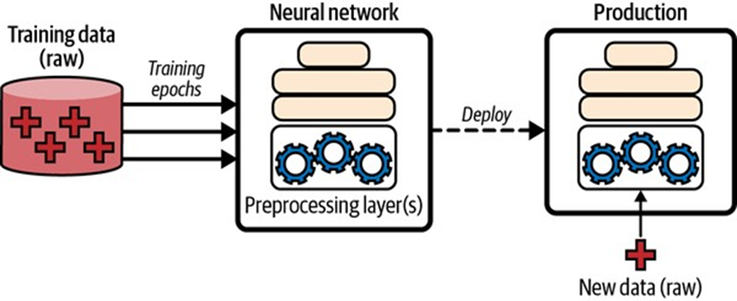
\includegraphics[width=\textwidth,height=0.65\textheight,keepaspectratio]{../machineLearningWeb/Figures/CH13/Hình_13-4}
            \vspace{0.2cm}
            \textit{Hình 13-4: Bao gồm các lớp tiền xử lý bên trong một mô hình}
        \end{column}
    \end{columns}
\end{frame}

\begin{frame}{Tiền Xử Lý Một Lần (AOT Preprocessing)}
    \begin{columns}
        \begin{column}{0.5\textwidth}
            \begin{itemize}
                \item Khuyết điểm của cách nhúng: Mỗi epoch đều phải tính lại Standardization $\rightarrow$ lãng phí.
                \item Tối ưu: Dùng tf.data để chạy lớp chuẩn hóa \textbf{một lần} toàn bộ dữ liệu (lưu ra cache).
                \item Khi xuất mô hình (Export) cho người dùng cuối, ta mới gắn lại lớp Tiền xử lý vào mô hình.
                \item \textbf{Hình 13-5} minh họa quy trình kép thông minh này.
            \end{itemize}
        \end{column}
        \begin{column}{0.5\textwidth}
            \centering
            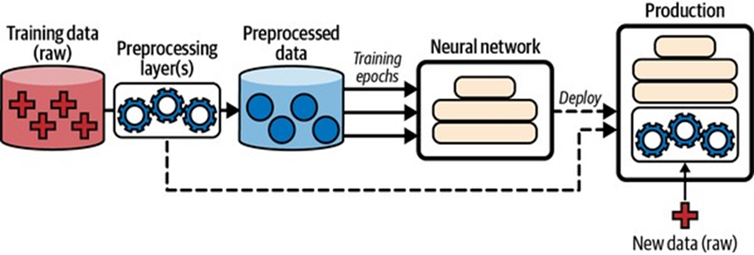
\includegraphics[width=\textwidth,height=0.65\textheight,keepaspectratio]{../machineLearningWeb/Figures/CH13/Hình_13-5}
            \vspace{0.2cm}
            \textit{Hình 13-5: Tiền xử lý dữ liệu một lần trước khi huấn luyện}
        \end{column}
    \end{columns}
\end{frame}

\begin{frame}[fragile]{Chuẩn Hóa Dữ Liệu (Normalization)}
    Keras cung cấp lớp \texttt{Normalization} thực hiện $x' = (x - \mu) / \sigma$.
\begin{lstlisting}[language=Python]
norm_layer = keras.layers.Normalization()

# Tinh toan (adapt) Mean va Variance truoc tren tap Train
norm_layer.adapt(X_train)

# Ap dung
X_train_scaled = norm_layer(X_train)

# Dua vao model
model = keras.models.Sequential([
    norm_layer,
    keras.layers.Dense(1)
])
\end{lstlisting}
\end{frame}

\begin{frame}[fragile]{Rời Rạc Hóa Dữ Liệu Liên Tục (Discretization)}
    \begin{itemize}
        \item Biến dữ liệu số thực thành dạng hạng mục (Categorical bins).
        \item Vd: Tuổi (24, 30, 45, 60) thành các nhóm (<25, 25-50, >50).
    \end{itemize}
\begin{lstlisting}[language=Python]
discretization_layer = keras.layers.Discretization(bin_boundaries=[25., 50.])

# 24 -> bin 0
# 30, 45 -> bin 1
# 60 -> bin 2
\end{lstlisting}
\end{frame}

\section{5. Tiền xử lý Biến Phân Loại (Categorical Features)}

\begin{frame}{Mã Hóa One-Hot (One-Hot Encoding)}
    \begin{itemize}
        \item Biến phân loại (ví dụ: Nghề nghiệp = "Kỹ sư", "Bác sĩ", "Giáo viên").
        \item Neural network không hiểu chuỗi văn bản.
        \item Mã hóa One-hot chuyển chúng thành vector nhị phân. "Kỹ sư" = [1, 0, 0]. "Bác sĩ" = [0, 1, 0].
    \end{itemize}
\end{frame}

\begin{frame}[fragile]{StringLookup và CategoryEncoding}
    \begin{itemize}
        \item Trước hết, cần xây dựng từ điển (Vocabulary) ánh xạ chuỗi thành số nguyên (StringLookup).
        \item Sau đó, biến số nguyên thành One-Hot (CategoryEncoding).
    \end{itemize}
\begin{lstlisting}[language=Python]
vocab = ["<1H OCEAN", "INLAND", "NEAR OCEAN", "NEAR BAY", "ISLAND"]
# string_lookup se anh xa chuoi vao cac so 0, 1, 2...
lookup_layer = keras.layers.StringLookup(vocabulary=vocab)

# encoded = CategoryEncoding
cat_encoding_layer = keras.layers.CategoryEncoding(num_tokens=lookup_layer.vocab_size())
\end{lstlisting}
\end{frame}

\begin{frame}{Hạn Chế của One-Hot Encoding}
    \begin{itemize}
        \item Nếu biến phân loại có quá nhiều giá trị (ví dụ: Tên 100,000 thành phố), mã hóa One-Hot sẽ tạo ra một vector khổng lồ dài 100,000 phần tử, toàn là số 0, chỉ có duy nhất một số 1.
        \item Lãng phí bộ nhớ khủng khiếp.
        \item Mạng nơ-ron phải nhân vô số trọng số dư thừa bằng 0.
        \item Giải pháp: \textbf{Embedding}.
    \end{itemize}
\end{frame}

\section{6. Embeddings (Nhúng)}

\begin{frame}{Khái Niệm Nhúng (Embedding)}
    \begin{columns}
        \begin{column}{0.5\textwidth}
            \begin{itemize}
                \item Embedding là một vector nhỏ, liên tục (thường từ 10 đến 300 chiều) đại diện cho một danh mục.
                \item Thay vì mã hóa cố định (như One-hot), giá trị trong vector Embedding \textbf{có thể được học} và điều chỉnh qua quá trình backpropagation!
                \item \textbf{Hình 13-6} (trái): Bắt đầu khởi tạo ngẫu nhiên, các danh mục nằm rải rác.
                \item \textbf{Hình 13-6} (phải): Sau khi huấn luyện, các danh mục có ý nghĩa giống nhau tụ lại gần nhau ("NEAR BAY" và "NEAR OCEAN").
            \end{itemize}
        \end{column}
        \begin{column}{0.5\textwidth}
            \centering
            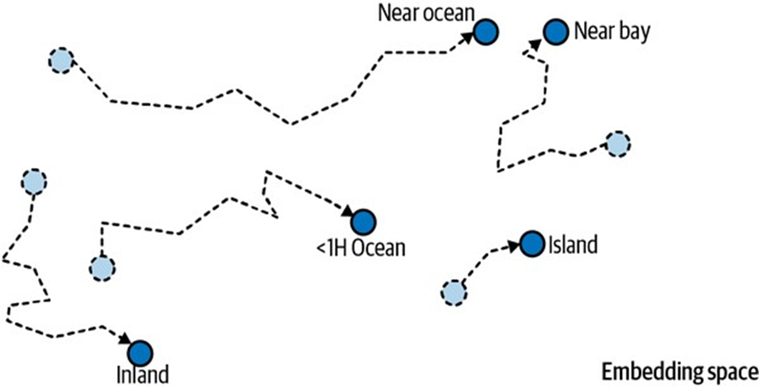
\includegraphics[width=\textwidth,height=0.7\textheight,keepaspectratio]{../machineLearningWeb/Figures/CH13/Hình_13-6}
            \vspace{0.2cm}
            \textit{Hình 13-6: Quá trình tự động cải thiện Embedding}
        \end{column}
    \end{columns}
\end{frame}

\begin{frame}{Không Gian Ngữ Nghĩa của Word Embeddings}
    \begin{columns}
        \begin{column}{0.5\textwidth}
            \begin{itemize}
                \item Tính năng vĩ đại nhất của Nhúng Từ (Word Embedding).
                \item Mạng tự học cách mã hóa \textbf{khái niệm} vào không gian.
                \item \textbf{Hình 13-7}: Trong Word2Vec, khoảng cách (Man, Woman) gần như tương đương với (King, Queen).
                \item Phép tính đại số từ vựng: $King - Man + Woman \approx Queen$.
            \end{itemize}
        \end{column}
        \begin{column}{0.5\textwidth}
            \centering
            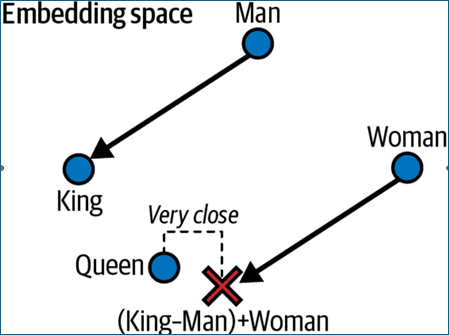
\includegraphics[width=\textwidth,height=0.65\textheight,keepaspectratio]{../machineLearningWeb/Figures/CH13/Hình_13-7}
            \vspace{0.2cm}
            \textit{Hình 13-7: Trục Không gian ngữ nghĩa (giới tính)}
        \end{column}
    \end{columns}
\end{frame}

\begin{frame}[fragile]{Code: Xây Dựng Embedding trong Keras}
\begin{lstlisting}[language=Python]
vocab_size = 1000  # 1000 tu vung
embed_size = 2     # Vector gom 2 chieu (de de ve do thi)

# Lop embedding hoat dong nhu mot bang tra cuu
embed_layer = keras.layers.Embedding(input_dim=vocab_size, output_dim=embed_size)

model = keras.models.Sequential([
    keras.layers.StringLookup(vocabulary=vocab),
    embed_layer,
    keras.layers.Dense(1)
])
\end{lstlisting}
\end{frame}

\section{7. TF Transform và TF Datasets}

\begin{frame}{TensorFlow Transform (tf.Transform)}
    \begin{itemize}
        \item Nhược điểm của việc dùng TF để tính Mean/Var cho tập Train là phải quét toàn bộ tập dữ liệu. Nếu dữ liệu quá lớn, việc này tốn rất nhiều thời gian.
        \item \textbf{TF Transform (tft)} ra đời cho việc Tiền xử lý quy mô cực lớn (ví dụ: chạy trên cụm Apache Spark, Apache Beam).
        \item Hàm tiền xử lý tft có thể chạy trên đám mây để chuẩn hóa hàng Terabyte dữ liệu.
        \item Sau đó tft sinh ra một TENSORFLOW GRAPH chứa sẵn công thức tiền xử lý (các hằng số mean, std) để nhúng vào mô hình khi Serving.
    \end{itemize}
\end{frame}

\begin{frame}{TensorFlow Datasets (TFDS)}
    \begin{itemize}
        \item Google cung cấp kho dữ liệu khổng lồ chuẩn bị sẵn: \textbf{TensorFlow Datasets}.
        \item Bao gồm hàng trăm dataset nổi tiếng: MNIST, CIFAR10, IMDB, Wikipedia, ImageNet.
    \end{itemize}
\end{frame}

\begin{frame}[fragile]{Sử dụng TFDS}
\begin{lstlisting}[language=Python]
import tensorflow_datasets as tfds

# Tu dong tai ve, tien xu ly va tra ve tf.data.Dataset
dataset = tfds.load(name="mnist", split="train")

# Truc tiep dua vao model
dataset = dataset.shuffle(10000).batch(32).prefetch(1)
for item in dataset:
    images = item["image"]
    labels = item["label"]
    # ...
\end{lstlisting}
\end{frame}

\section{Tổng Kết}

\begin{frame}{Tổng Kết Chương 13}
    \begin{itemize}
        \item \textbf{tf.data API:} Công cụ vô song để xây dựng đường ống dữ liệu (pipeline). Hỗ trợ đọc từ nhiều file song song (interleave), trộn (shuffle), và tăng tốc bằng prefetching.
        \item \textbf{TFRecord:} Định dạng nhị phân gọn nhẹ của TensorFlow.
        \item \textbf{Keras Preprocessing Layers:} Cung cấp cơ chế nhúng lớp tiền xử lý trực tiếp vào Mô hình (Normalization, StringLookup...).
        \item \textbf{Embeddings:} Kỹ thuật vĩ đại biểu diễn chuỗi/danh mục bằng vector số thực, tự động học ra ngữ nghĩa trong không gian liên tục (thay cho One-Hot Encoding lãng phí).
    \end{itemize}
\end{frame}

\end{document}
